%-------------------------------
%-------------------------------
\chapter{Zusätzliche Funktionen}
\label{chapter:additional_features}


%---------------------------
\section{Benutzeroberfläche}
\label{gui}

Mit dem in Kapitel \ref{chapter:skeleton_generation} vorgestellen Algorithmus können nicht nur zufällige Skelette generiert werden. Über eine Benutzeroberfläche ist es auch möglich dem Algorithmus zusätzliche Eingaben zu geben. Die Benutzeroberfläche ist in Abbildung \ref{gui_screenshot} zu sehen.
Im Folgenden ist für alle möglichen Eingaben beschrieben, wie sie in Bedingungen für die PCA umgesetzt werden. Ist in Zahlenfeldern nichts eingegeben, haben diese keinen Einfluss auf den Ablauf (im Gegensatz zur Eingabe der Zahl $0$).

\begin{figure}
 \centering
 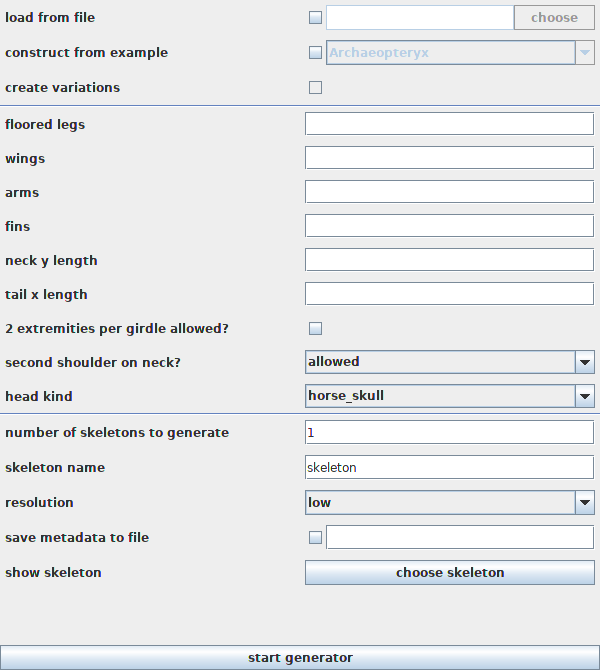
\includegraphics[width=0.7\textwidth]{graphics/gui.png}
 \caption{Die Benutzeroberfläche des Programms. Der Knopf "`start generator"' startet den Algorithmus mit den zusätzlichen Eingaben aus den Feldern darüber.}
 \label{gui_screenshot}
\end{figure}

\begin{itemize}
 \item Die Anzahl der Beine mit Bodenkontakt (floored legs) muss eine gerade Zahl $n$ zwischen $0$ und $8$ sein. Die Hälfte wird als Bedingung für \emph{Paare von Beinen mit Bodenkontakt} an die PCA weitergegeben, wie in Abschnitt \ref{pca_conditions} beschrieben. Bei echten Wirbeltieren liegt die Anzahl der Beine zwischen $0$ und $4$. Werden Werte größer $4$ als Bedingung an die PCA gestellt, so werden sehr stark geschwungene Wirbelsäulen generiert. Diese sehen aber, bis zu einem Wert von ca.\ $8$ gar nicht schlecht aus (siehe Abbildung \ref{more_extremities} a). Deshalb werden diese Werte auch als Bedingungen erlaubt. Sie werden nur mit einer gewissen Wahrscheinlichkeit etwas verkleinert, weil fantastische Tiere mit mehr als $4$ Beinen auch mit Wirbelsäulen für Tiere mit $4$ Beinen generiert werden können.
 
 \item Die Anzahl der Flügel (wings) muss ebenfalls gerade sein. Die Hälfte des Eingabewerts, aber maximal $1$, wird als Bedingung an die PCA weitergegeben.
 Im Gegensatz zu den Beinen sind die Wirbelsäulen, die unter Bedingungen größer $1$ für \emph{Flügel} generiert werden, mit großer Wahrscheinlichkeit unrealistisch (siehe Abbildung \ref{more_extremities} b).
 
 \item Die Zahlen für Arme (arms) und Flossen (fins) gehen nicht als Bedingung in die PCA ein.
 
 \item Die $y$-Komponente des Abstands zwischen Kopf und Schultergürtel (neck $y$ length) und die $x$-Komponente des Abstands zwischen Hüfte und Schwanzspitze (tail $x$ length) können wiederum direkt als Bedingung an die PCA weitergegeben werden. Auch hier werden, wie auch bei Beinen und Flügeln (wie in Abschnitt \ref{pca_conditions} beschrieben), zufällige kleine Werte aufaddiert oder abgezogen um mehr Variation auf den erzeugten Skeletten zu bekommen.
\end{itemize}

\begin{figure}
 \subfloat[$8$ Beine]{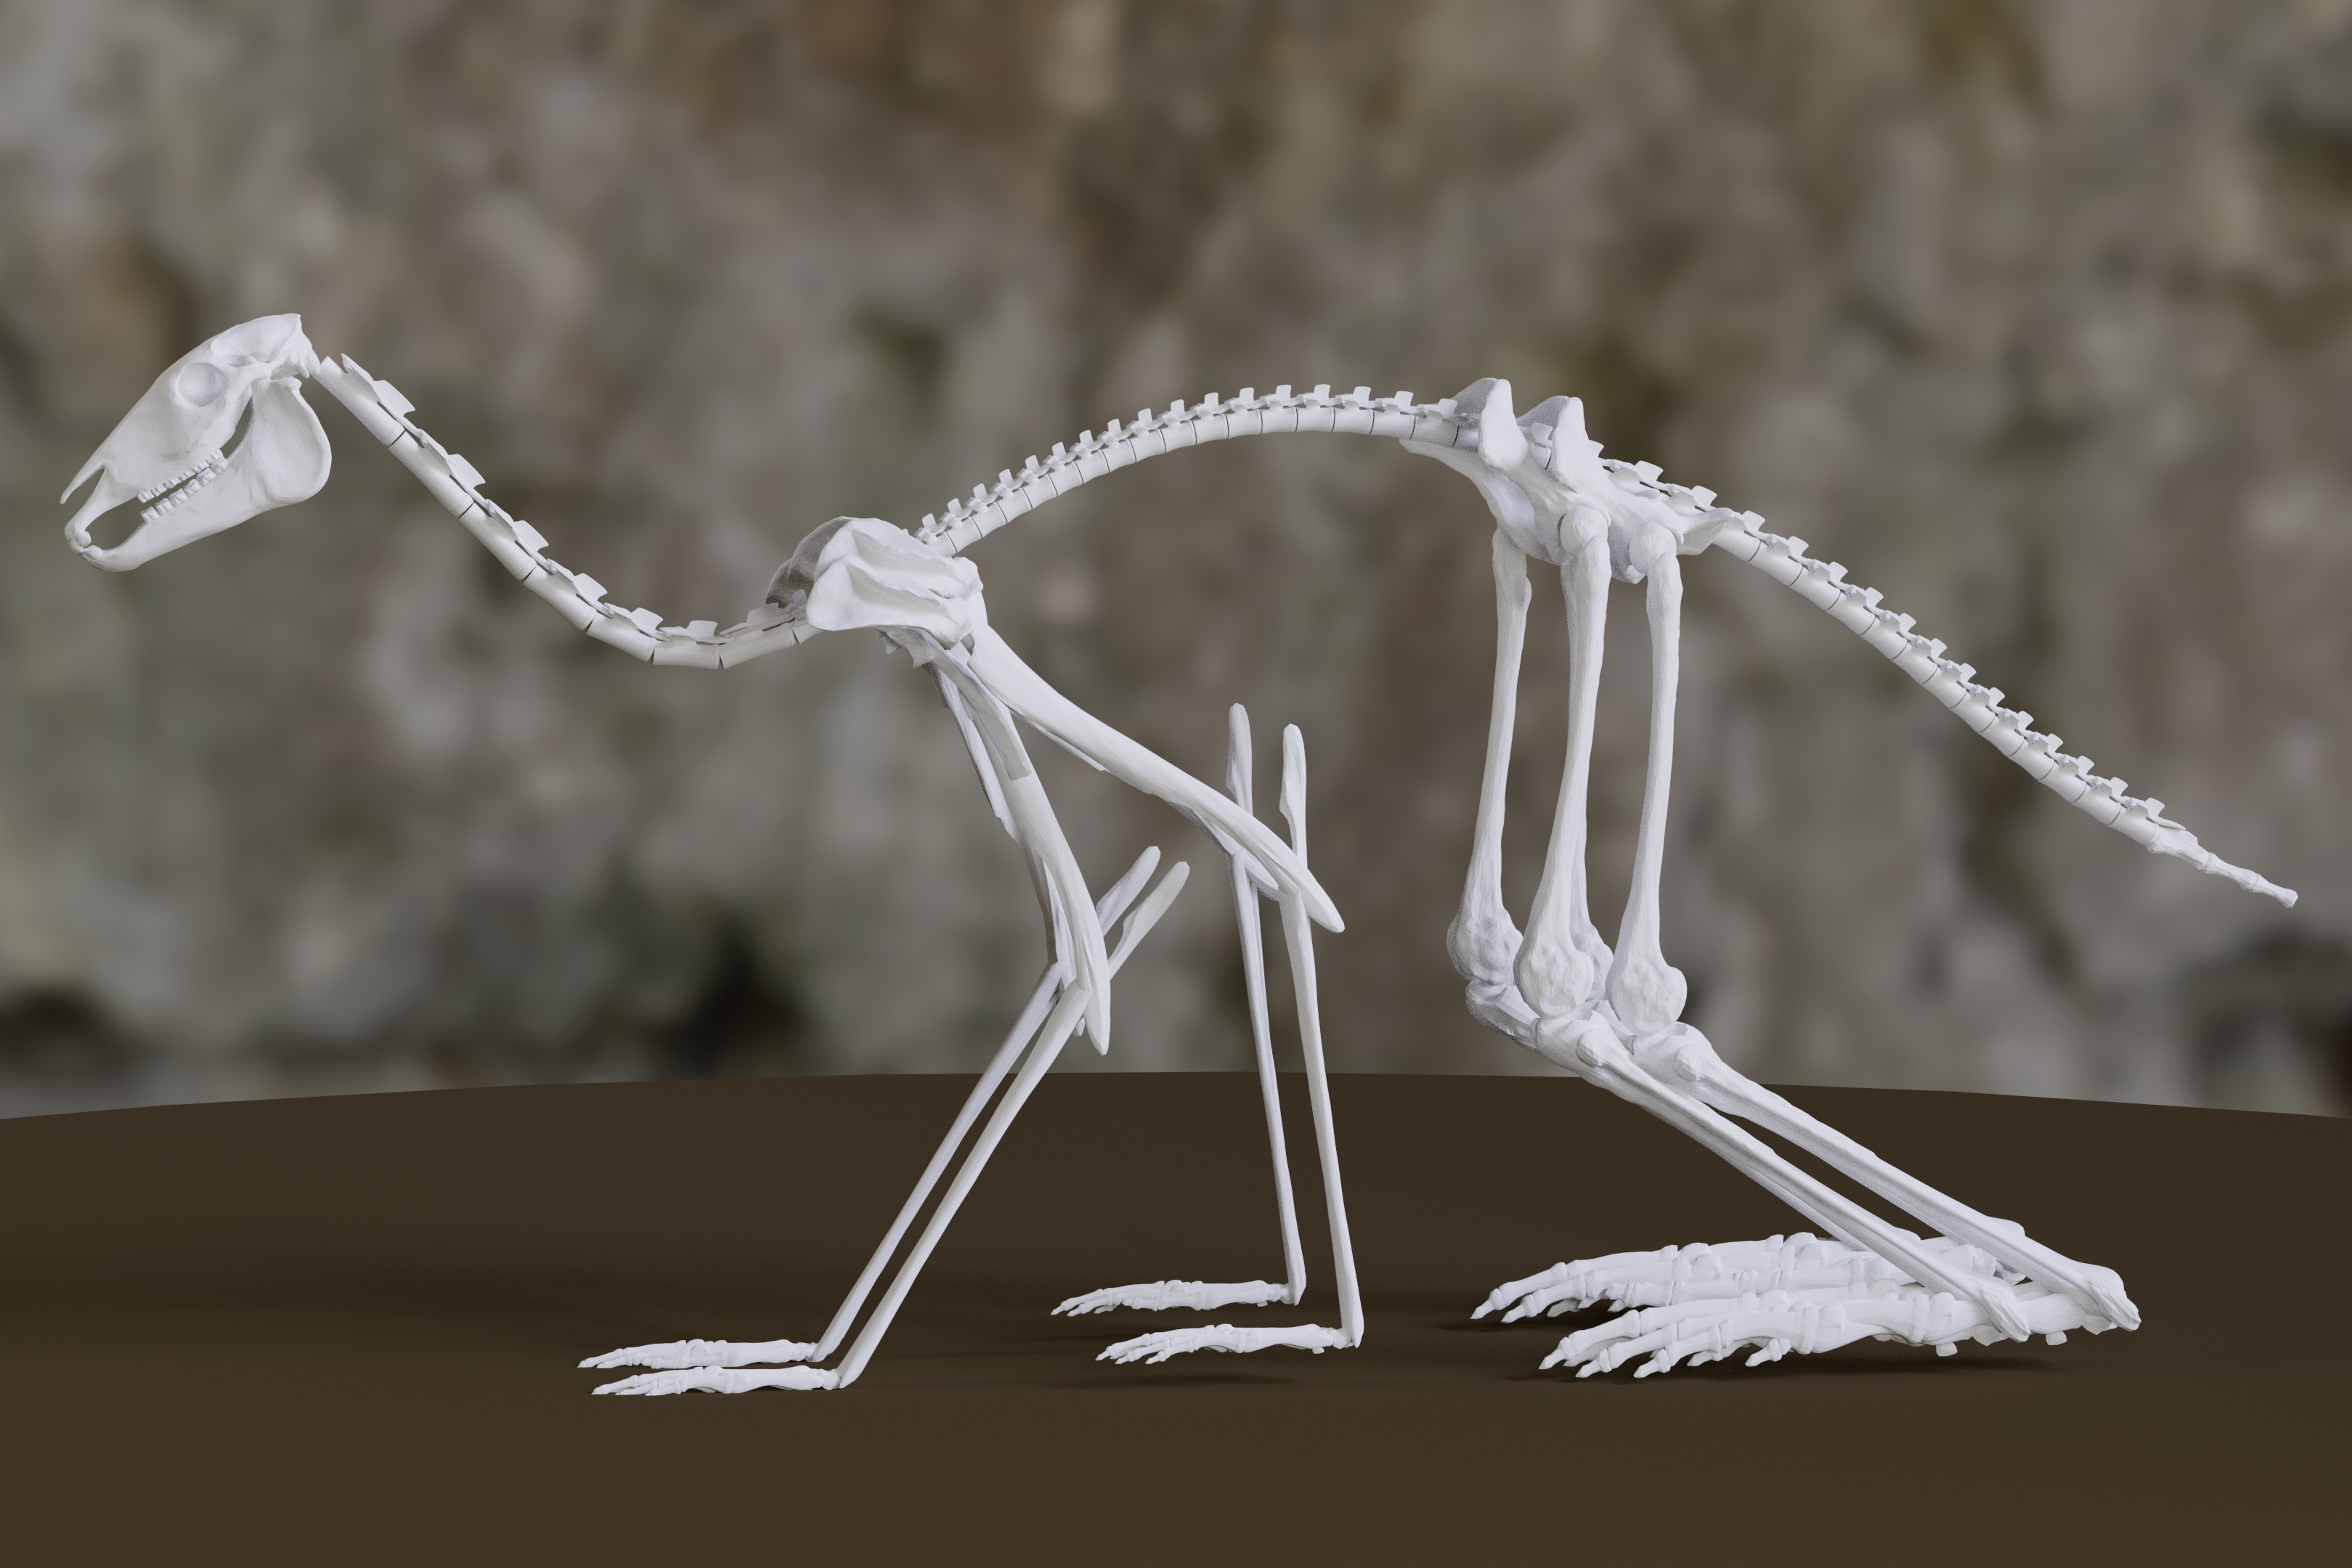
\includegraphics[height=5.8cm]{../java_skeleton_generation/example_skeletons/8legs.jpg}}~
 \subfloat[$1{,}5$ Flügel]{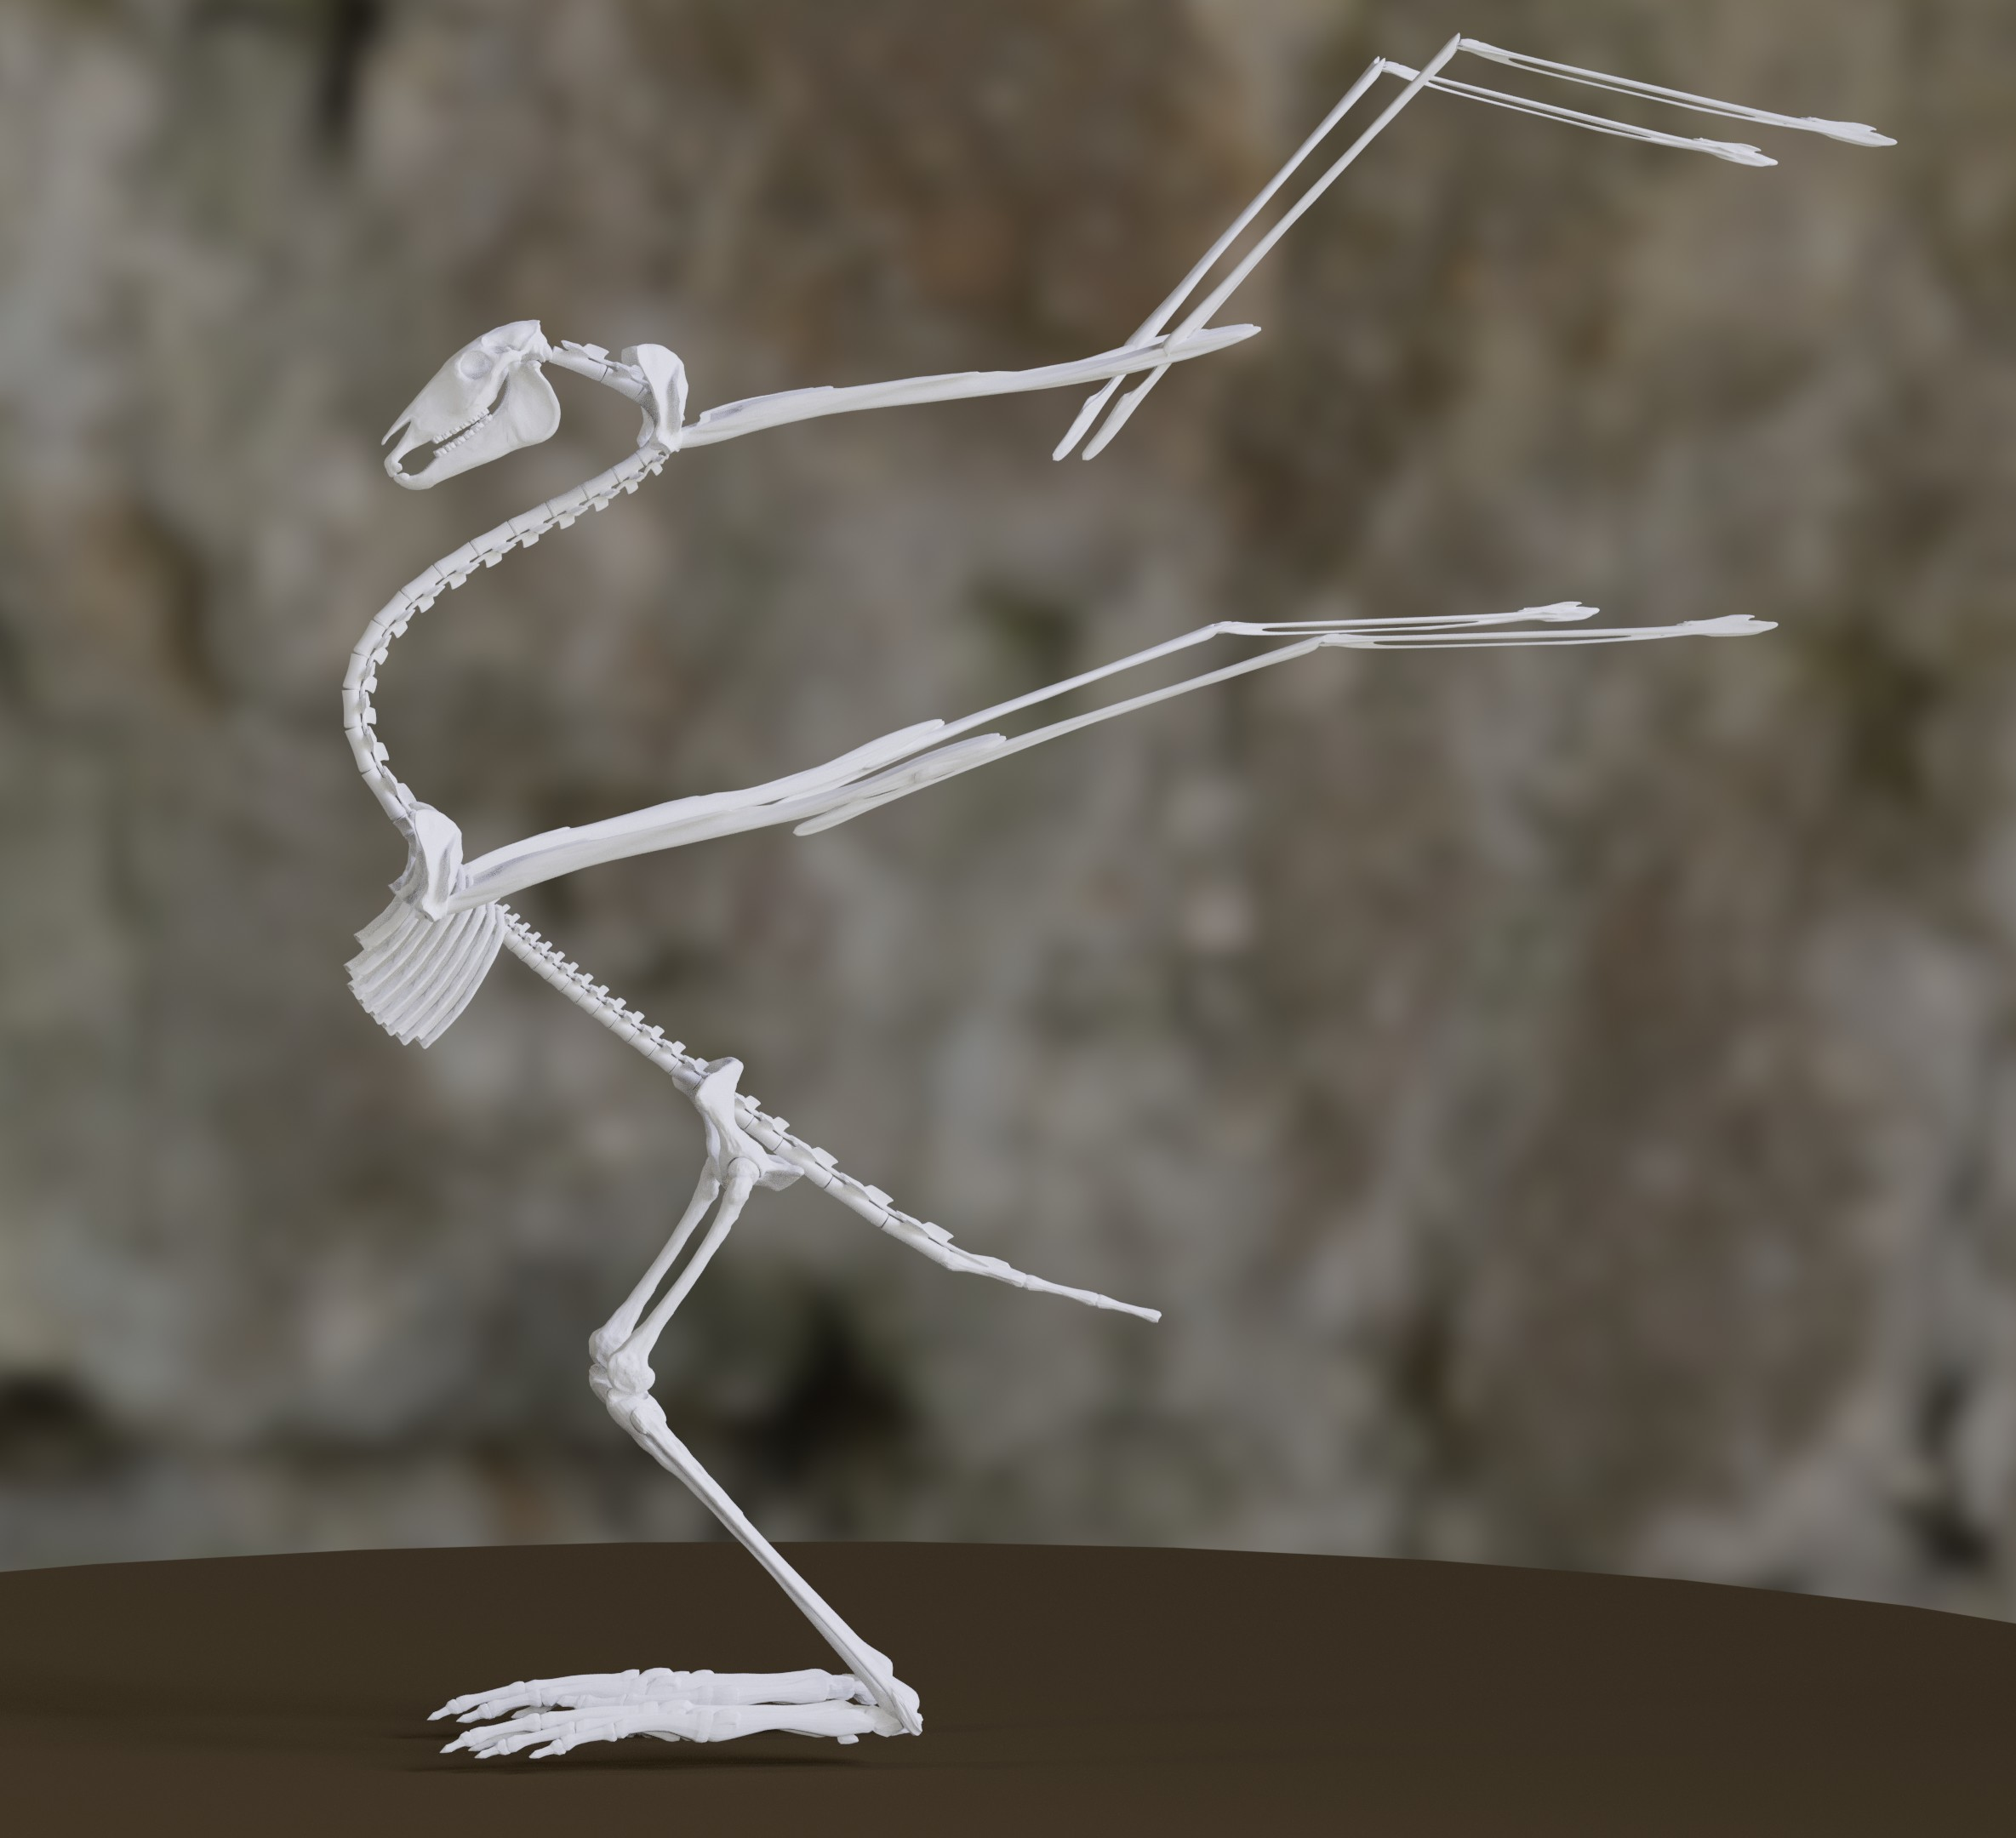
\includegraphics[height=5.8cm]{../java_skeleton_generation/example_skeletons/15wings.jpg}}
 
 \caption{Zwei Skelette, die mit extremen Bedingungen für die PCA generiert wurden. (a) Benutzereingabe: $8$ Beine und $4$ Beinpaare als Bedingung für die PCA. Es ist kein zweiter Schultergürtel am Hals erlaubt, aber zwei Extremitätenpaare pro Extremitätengürtel. (b) Benutzereingabe $4$ Flügel und $1{,}5$ Flügelpaare als Bedingung für die PCA. Ein zweiter Schultergürtel am Hals wird erzwungen, aber es ist nur ein Extremitätenpaar pro Extremitätengürtel erlaubt. Skelette, die mit einer Bedingung von $2$ Flügelpaaren generiert werden, haben einen Hals, der noch extremer geschwungen ist.}
 \label{more_extremities}
\end{figure}


Die Anzahlen der verschiedenen Extremitätentypen werden außerdem verwendet um die Parameter $e_v, e_h$ und $e_{v2}$ für die Anzahl der Vorder- und Hinterextremitäten der Grammatik (siehe Abschnitte \ref{section:grammar} und \ref{additional_extremities}) zu bestimmen und um den Typ und damit die Positionierung der verschiedenen generierten Extremitäten festzulegen (siehe Anfang \mbox{Abschnitt \ref{section:extremity_generation}}). Zusätzlich muss mit einberechnet werden ob zwei Extremitätenpaare pro Extremitätengürtel erlaubt sind ($2$ extremities per girdle allowed?) und ob ein zweiter Schultergürtel auf dem Hals erlaubt, erzwungen oder verboten ist (second shoulder on neck?) (siehe auch Abschnitt \ref{additional_extremities}).

% Modell für Kopf
Außerdem gibt es theoretisch noch die Möglichkeit anzugeben welches 3D-Modell für den Kopf verwendet werden soll (head kind). Leider gibt es hier, Stand Abschluss der Arbeit, nur eines zu Auswahl. Dies ließe sich aber leicht anpassen (siehe Abschnitt \ref{bone_models}).
Zusätzlich kann eingestellt werden welche Auflösung das 3D-Modell haben soll (resolution). Hier gibt es die Möglichkeit nur Quader zu generieren oder Modelle von echten Knochen in niedriger oder hoher Auflösung einzusetzen.

% Dateiname, Anzahl und JavaView
Im Feld "`skeleton name"' kann der Dateiname des zu generierenden Modells eingestellt werden und in "`number of skeletons to generate"' kann festgelegt werden wieviele Skelette auf einmal generiert werden sollen. Und schließlich kann man sich auch ein generiertes Modell anzeigen lassen (show skeleton). Dazu wird das Programm \emph{JavaView} \cite{JavaView} verwendet. Es ist darauf spezialisiert 3D-Geometrie interaktiv zu visualisieren und kann in Javacode eingebunden werden.


%------------------------------------------
\section{Speichern und Laden von Skeletten}
\label{load_skeletons}

Um ein vorgegebenes Skelett reproduzieren zu können reicht es einige Metadaten zu speichern. Dazu gehören die Dimensionen der PCA (Position der Wirbelsäule, Länge der Knochen in den Extremitäten und Gewicht) und Daten, die zusätzlich generiert werden (Anzahl und Art der Extremitäten an den jeweiligen Extremitätengürteln, die Winkel an den Gelenken der Extremitäten, Anzahl der Wirbel und Rippen und welches 3D-Modell für den Kopf verwendet werden soll).
Das alles wird in wenigen Java-Klassen gebündelt. So können die Daten über Java-Serialisierung \cite{JavaSerialization} in eine Textdatei geschrieben werden. Diese Datei kann dann wieder eingelesen werden um die Klassen wieder herzustellen.

% gui
Im Benutzerinterface (Abbildung \ref{gui_screenshot}) kann diese Funktion verwendet werden, indem "`save metadata to file"' ausgewählt wird und ein Dateiname eingegeben wird. Dann wird für jedes generierte Skelett eine Textdatei mit dem angegebenen Namen generiert, die die serialisierten Daten enthält.\\
Um ein Skelett aus solch einer Textdatei zu laden, muss die entsprechende Datei bei "`load from file"' ausgewählt werden. Dann werden die dazugehörigen Java-Klassen wieder hergestellt und das gleiche 3D-Modell noch einmal generiert.

% kein metadaten nach außen
Das funktioniert natürlich nur über das implementierte Programm, das genau die serialisierten Java-Klassen enthält und liefert keine Zusatzinformationen zu dem generierten Skelett an den Benutzer. Solche Zusatzinformationen könnten hilfreich für die Weiterverarbeitung des erzeugten Modells sein. In weiterführenden Arbeiten könnten sie zusätzlich generiert werden. Hilfreiche Informationen könnten dabei \zb die Knochenhierarchie oder die Winkeleinschränkungen an den Gelenken sein.

% pca Beispiele laden
Zusätzlich gibt es die Funktion konkrete PCA-Eingabebeispiele auszuwählen (construct from example). Dann wird ein Skelett mit den Daten generiert, die für dieses Beispiel erhoben wurden. Mit einem PCA-Punkt sind aber noch nicht alle Daten festgelegt, die ein Skelett bestimmen. Es ist nur festgelegt welcher PCA-Punkt in Schritt 2 des Algorithmus ausgewählt wird, nicht welche konkreten Parameter die Grammatik bekommt oder welche Typen von Extremitäten generiert werden (siehe Abschnitt \ref{section:overview}). Deshalb ist es zusätzlich möglich weitere Bedingungen \zb für die Anzahl der Arme anzugeben.


%----------------------------------
\section{Erzeugung von Variationen}

Sucht man Inspiration zu einem bestimmten Typ von Skelett oder Tier, so kann es hilfreich sein Variationen zu einem vorgegebenen Skelett generieren zu können. 
Vielleicht wurde ein interessantes Skelett generiert und man möchte dazu schnell viele ähnliche Skelette finden.
Dies ist relativ leicht mit dem hier vorgestellten Algorithmus möglich. In der Benutzeroberfläche muss "`create variations"' ausgewählt werden.

% was ist gegeben
Als Grundlage für Variationen kann ein gespeichertes Skelett oder ein Eingabebeispiel der PCA dienen (siehe Abschnitt \ref{load_skeletons}). Es ist also mindestens ein Punkt mit den erhobenen Merkmalen für die PCA gegeben. Bei einem gespeicherten Skelett ist zusätzlich noch gegeben wieviele Wirbel, Rippen und Extremitäten generiert werden und welche Art von Extremität an welchem Ansatzpunkt beginnt.
Ist nur ein Eingabebeispiel der PCA gegeben, so fehlen diese Angaben. Es werden aber zusätzlich Benutzereingaben, \zb zur Anzahl verschiedener Extremitätentypen, berücksichtigt.

% pca punkt variieren
Für die Variationen wird zwischen Eingabemerkmalen für die PCA und unabhängig generierten Daten unterschieden. Um Variationen von einem Punkt $p = (x_1, x_2,\dots, x_n)$ im PCA-Raum zu generieren, wird für jede Dimension eine neue Zufallszahl erzeugt. Dies ergibt dann einen Punkt $p' = (x_1', x_2',\dots,x_n')$. Ein $x_i'$ wird mit einer Normalverteilung zum Erwartungswert $x_i$ erzeugt.
Der konkrete Wert für die Varianz wurde experimentell bestimmt. Er sollte nicht zu groß sein, damit die generierten Skelette sich ähneln, aber auch nicht zu klein, damit sie sich etwas unterscheiden. In der Implementierung wird
die Hälfte der Varianz verwendet, die die PCA für Dimension $i$ berechnet hat, also die Hälfte des Eigenwerts, der zur $i$-ten Dimension gehört. 

% Rest variieren
Bei den Merkmalen, die unabhängig von der PCA sind, wird unterschiedlich vorgegangen. Die Anzahl der Wirbel und Rippen wird einfach neu zufällig bestimmt. Sie ist also unabhängig vom gegebenen Skelett.\\
Sind noch keine Ansatzpunkte und Arten von Extremitäten gegeben, werden diese zunächst berechnet. Danach wird ein Ansatzpunkt ausgelost, der verändert werden kann. Ist diesem Ansatzpunkt noch keine Extremität zugeteilt, wird mit Wahrscheinlichkeit $0{,}5$ eine zufällige Extremität, die an diesen Ansatzpunkt passt, hinzugefügt. Gibt es an dem Punkt schon eine Extremität, so wird diese, ebenfalls mit Wahrscheinlichkeit $0{,}5$ verändert. Bei einer Veränderung wird die Extremität an dem gewählten Ansatzpunkt gelöscht und mit einer gewissen Wahrscheinlichkeit\footnote{Im Code wurde hier eine Wahrscheinlichkeit von $0{,}2$ verwendet.} an einem anderen Punkt wieder eingefügt, falls möglich.\\
Danach werden die Skelettelemente durch die Grammatik neu generiert und dabei auch die Extremitäten neu positioniert.

\todo{generische Algorithmen zitieren (auch hinzufügen und löschen oder ändern von Features um Variationen/Verbesserungen zu erzeugen)}

